\documentclass[a4paper]{article}

\usepackage[english]{babel}
\usepackage[utf8]{inputenc}
\usepackage{amsmath}
\usepackage{graphicx}
\usepackage{color}
\usepackage{float}
\usepackage{listings}
\definecolor{keywords}{RGB}{255,0,90}
\definecolor{comments}{RGB}{0,0,113}
\definecolor{red}{RGB}{160,0,0}
\definecolor{green}{RGB}{0,150,0}
\definecolor{codegreen}{rgb}{0,0.6,0}
\definecolor{codegray}{rgb}{0.5,0.5,0.5}
\definecolor{codepurple}{rgb}{0.58,0,0.82}
\definecolor{backcolour}{rgb}{0.95,0.95,0.92}
\definecolor{brown}{rgb}{0.59, 0.29, 0.0}
\definecolor{beaublue}{rgb}{0.74, 0.83, 0.9}
\definecolor{orange}{rgb}{1.0, 0.5, 0.0}
\definecolor{darkslategray}{rgb}{0.18, 0.31, 0.31}
\definecolor{deepblue}{rgb}{0,0,0.5}
\definecolor{deepred}{rgb}{0.6,0,0}
\definecolor{deepgreen}{rgb}{0,0.5,0}
\definecolor{auburn}{rgb}{0.43, 0.21, 0.1}
\definecolor{bistre}{rgb}{0.24, 0.17, 0.12}
\definecolor{babyblue}{rgb}{0.54, 0.81, 0.94}
\definecolor{ballblue}{rgb}{0.13, 0.67, 0.8}
\lstdefinestyle{myMatlabstyle}{
	language=Matlab,
	backgroundcolor=\color{white},   
	commentstyle=\color{deepgreen},
	keywordstyle=\color{black},
	identifierstyle=\color{black},
	numberstyle=\tiny\color{codegray},
	stringstyle=\color{purple},
	basicstyle=\footnotesize,
	breakatwhitespace=false,         
	breaklines=true,                 
	captionpos=b,                    
	keepspaces=true,                 
	numbers=left,                    
	numbersep=5pt,                  
	showspaces=false,                
	showstringspaces=false,
	showtabs=false,                  
	tabsize=2
}
\lstdefinestyle{myPythonstyle}{
	language=Python, 
	basicstyle=\ttfamily\small, 
	keywordstyle=\color{blue},
	commentstyle=\color{green},
	stringstyle=\color{red},
	showstringspaces=false,
	identifierstyle=\color{black},
}
\lstset{language=Matlab,frame=single}
\lstset{language=Python,frame=single}
\usepackage[colorinlistoftodos]{todonotes}
\usepackage[scale=0.75]{geometry}
	\title{Principal Component Analysis: Dynamics of a paint can}

\author{Jithin D. George}

\date{\today}

\begin{document}
\maketitle

\begin{abstract}
This homework explores the implementation of the principal component analysis on the videos of an object. An exploration of the application of the PCA yields new perspectives on the underlying dynamics of the object.
\end{abstract}

\section{Introduction and Overview}
\label{sec:introduction}

The Principal Component Analysis is a technique from linear algebra that transform a matrix into its principal components. Each principal component captures most of the variation in the data while remaining orthogonal to and thus independent of the other components. When faced with an unknown data set, the PCA can look at the key components and offer new insights.
 
\section{Theoretical Background}
\label{sec:theory}

Suppose our data consists of measurements in the n dimensional space, the first principal component is an n-dimensional vector from which the variance of the measurements is minimized. Thus, by definition, it passes through the mean. The next component is obtained by removing all correlation with this first component. Thus, all the principal components are orthogonal.   
The SVD of a matrix decomposes it into three matrices.
\[A=USV^{*} \]
Here, U and V represent matrices of basis elements. S is the matrix of singular values. V could be considered as the original basis matrix. U would then be the principal component basis. 

The principal components can simply be obtained as 
\[T=U*S\]


\section{Implementation and Development}
The resource available to us are a set of video files documenting the motion of a paint can. Most of the code focuses on extracting relevant information from the video and tracking the paint can.

\subsection{Tracking the paint can}

I employed two methods to tracked the paint can 
\subsubsection{Average and spot}
\begin{itemize}
	\item Convert the image to greyscale
	\item Take the mean of all images (frames).
	\item Subtract the mean from all images.
	\item Filter out regions where the paint can won't go.
	\item Threshold the intensity.
	\item Use centroid to make clusters of the bright spots.
	\item Choose the center of the biggest cluster.
\end{itemize}

\subsubsection{White Edges}
\begin{itemize}
	\item Filter out regions where the paint can won't go.
	\item Find out the columns containing points where the maximum value in all red , green and blue are close to 255(white).
	\item Find the longest line( adjacent rows) of whiteness in all the columns.
	\item Choose the column as x and the mean of the rows as y.
	\item This corresponds to the left white edge of the paint can.
	\item In the case of the tilted cam 3, we use the rows instead of the columns.
	
\end{itemize}

The white edges method generated much more smooth curves than the averaging technique.


\subsection{The Principal Components}

We deal with data from 3 camera in both the x and y directions. That leads to 6 directions in total. We also consider 4 different cases - the ideal case, the noisy case and horizontal displacement and rotation.


The data for each case is converted to a 226x6 matrix. It is then normalized by dividing it by the maximum value (for each direction) and subtracting the mean(of each direction) from the matrix. This normalized matrix is subjected to the singular value decomposition. We then take a look at its principal components to get an idea of the dynamics of the paint can.




\section{Computational Results}

\subsection{The Ideal Case}

\subsubsection{The raw data}
After tracking the paint cans in all three videos, we get the following information

\begin{figure}[H] 
	\centering
	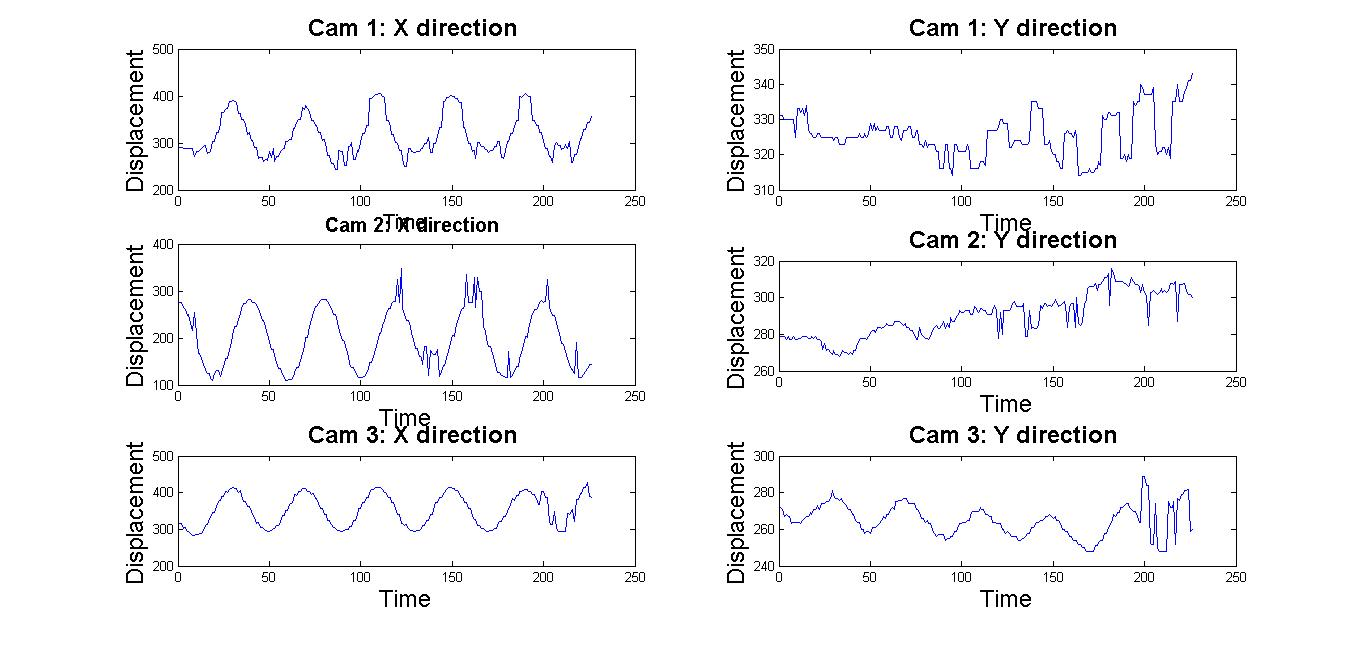
\includegraphics[width=0.7\textwidth]{rawdata.jpg}
	\caption{The raw data for the ideal case}	
\end{figure}


\subsubsection{The Percentage of variation captured}
\begin{figure}[h!] 
\centering
	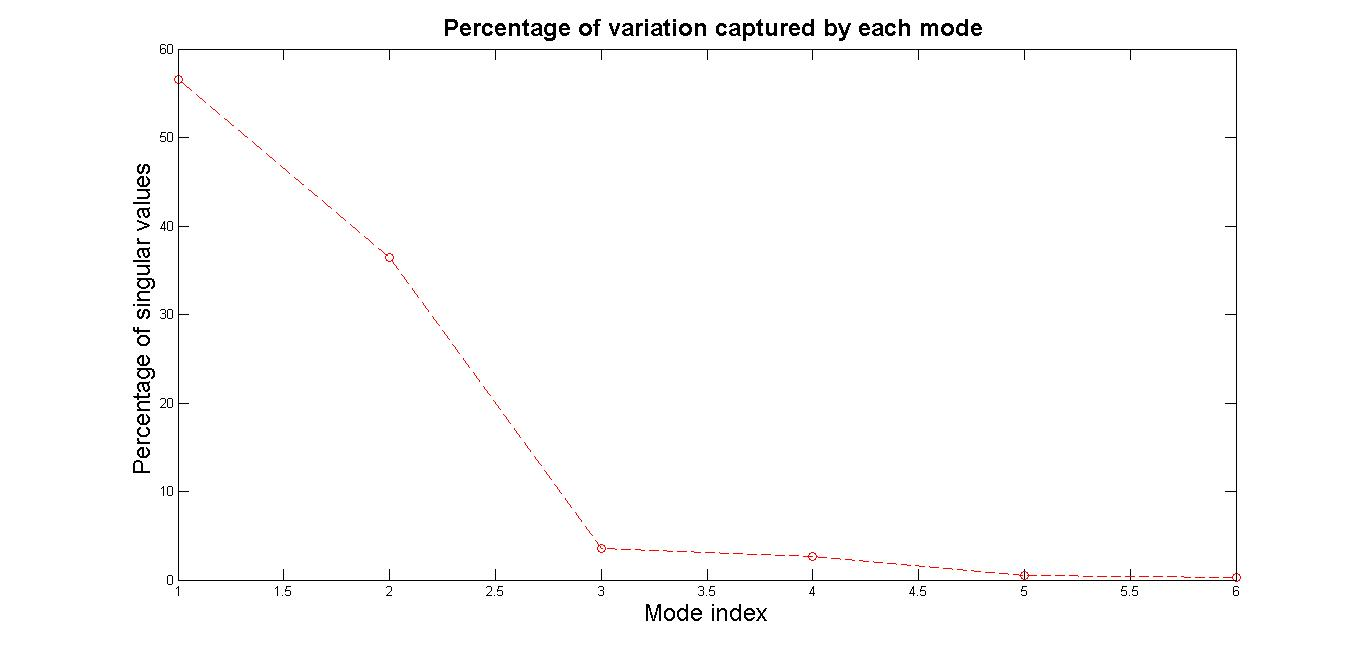
\includegraphics[width=0.8\textwidth]{percent1.jpg}
	\caption{The variation captured by each principal component}
\end{figure}

Nearly 60 percent of the data is captured by the first principal component. 

\subsubsection{The Principal Component}
\begin{figure}[H] 
	\centering
	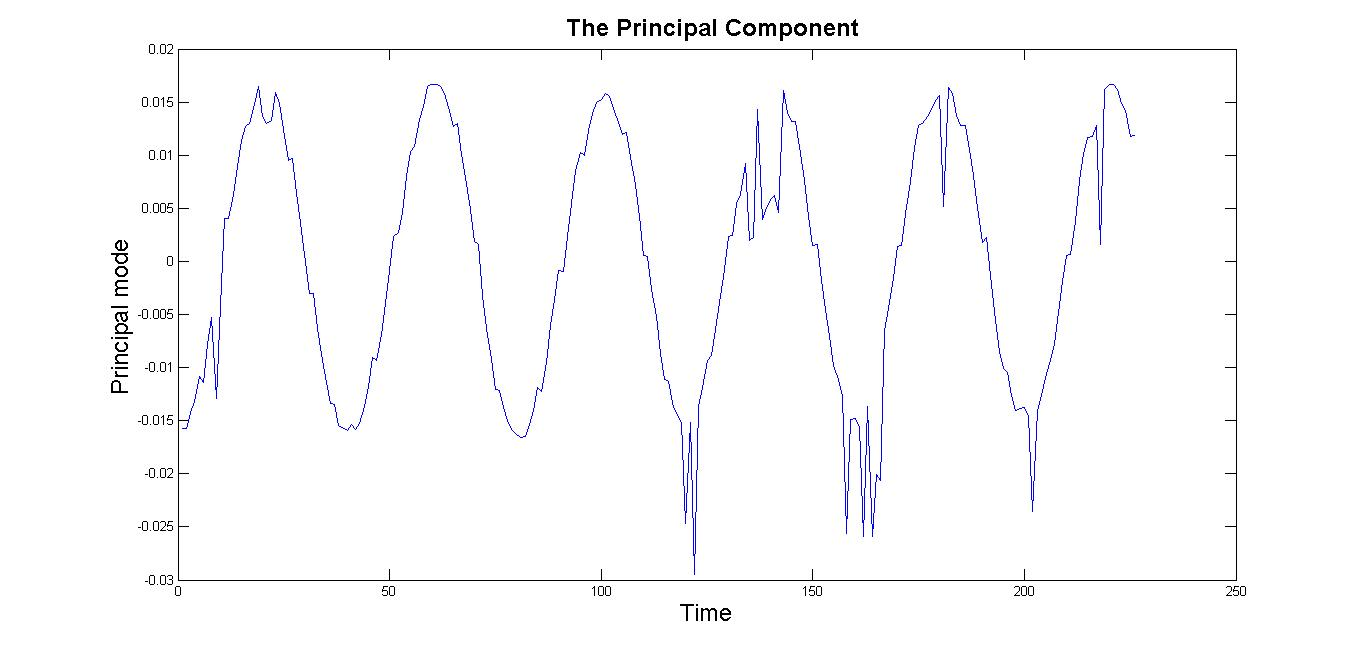
\includegraphics[width=0.8\textwidth]{PC1.jpg}
	
	\caption{The First Principal Component}	
\end{figure}
This is very close to the following equation
\[ y = A cos(wt+w_0)\]
The first mode captures the simple harmonic nature of the paint can with a little spikes.
\subsection{The Noisy Case}

\subsubsection{The raw data}
After tracking the paint cans in all three videos, we get the following information.

\begin{figure}[H] 
	\centering
	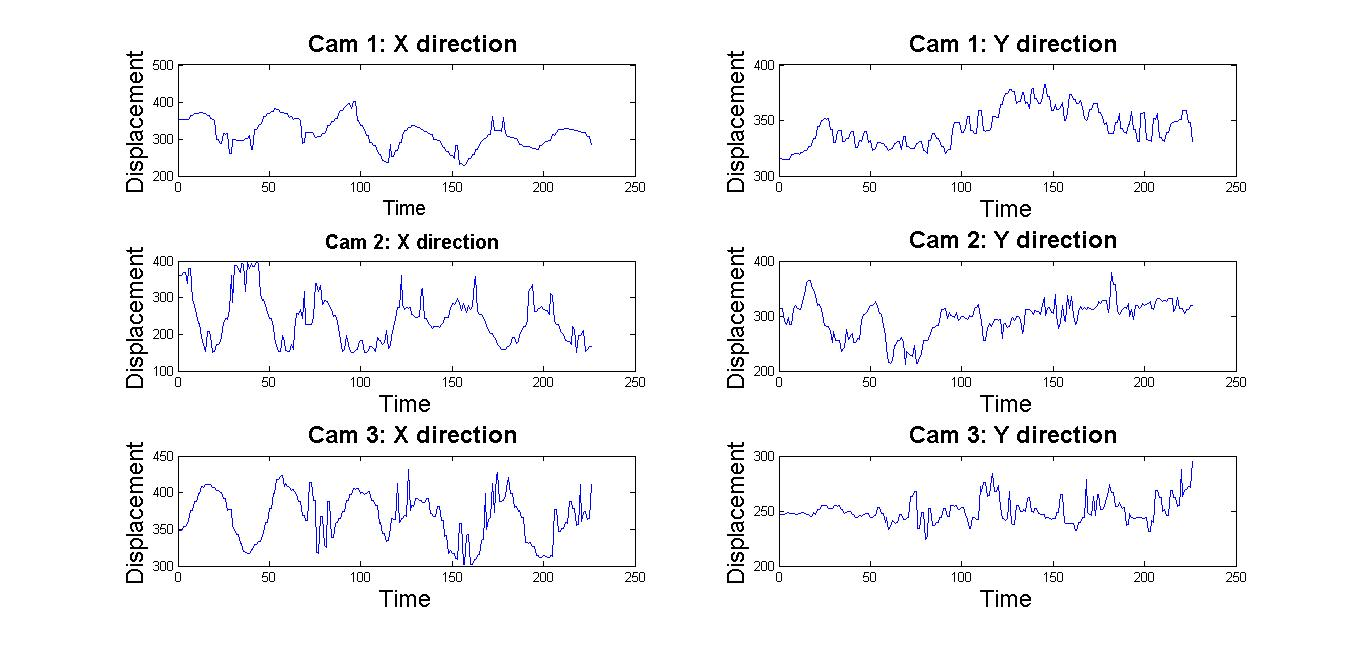
\includegraphics[width=0.8\textwidth]{rawdata2.jpg}
	\caption{The raw data for the noisy case}	
\end{figure}

There are lots of spikes in this data coming from the bad recording of the video.


\subsubsection{The Percentage of variation captured}
\begin{figure}[h!] 
	\centering
	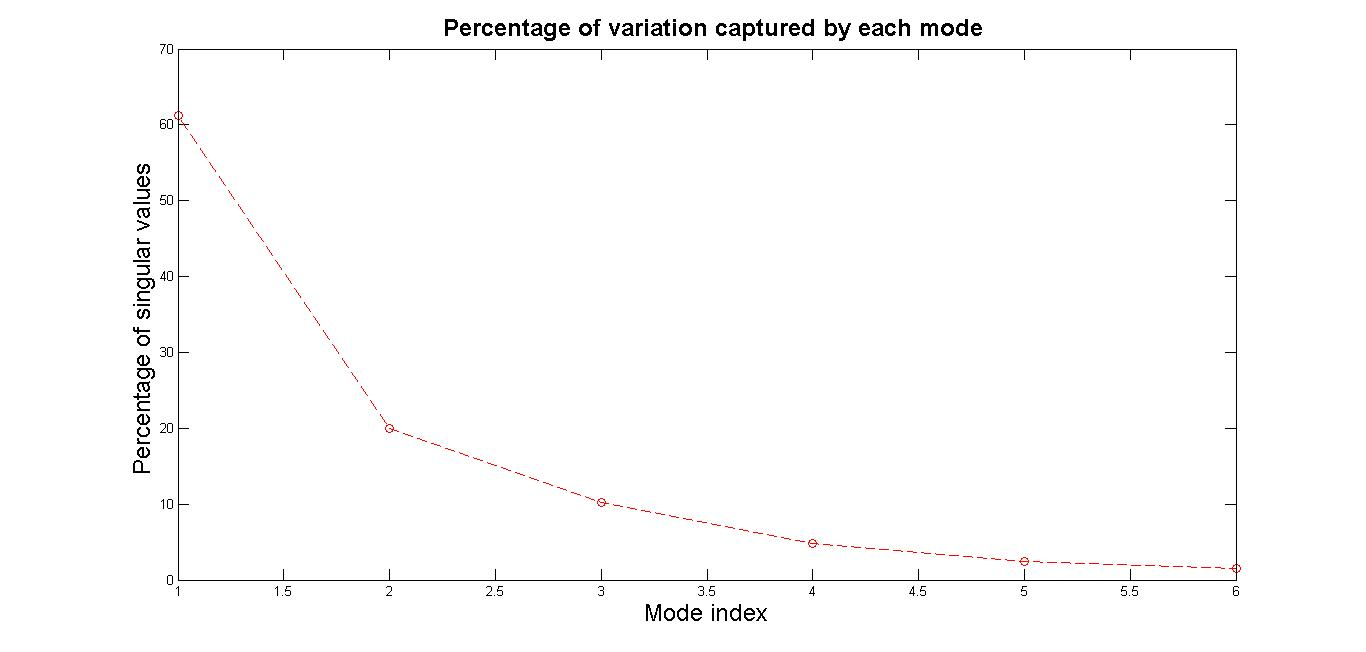
\includegraphics[width=0.6\textwidth]{percent2.jpg}
	\caption{The variation captured by each principal component}
\end{figure}

Over 60 percent of the data is captured by the first principal component. 

\subsubsection{The Principal Component}
\begin{figure}[H] 
	\centering
	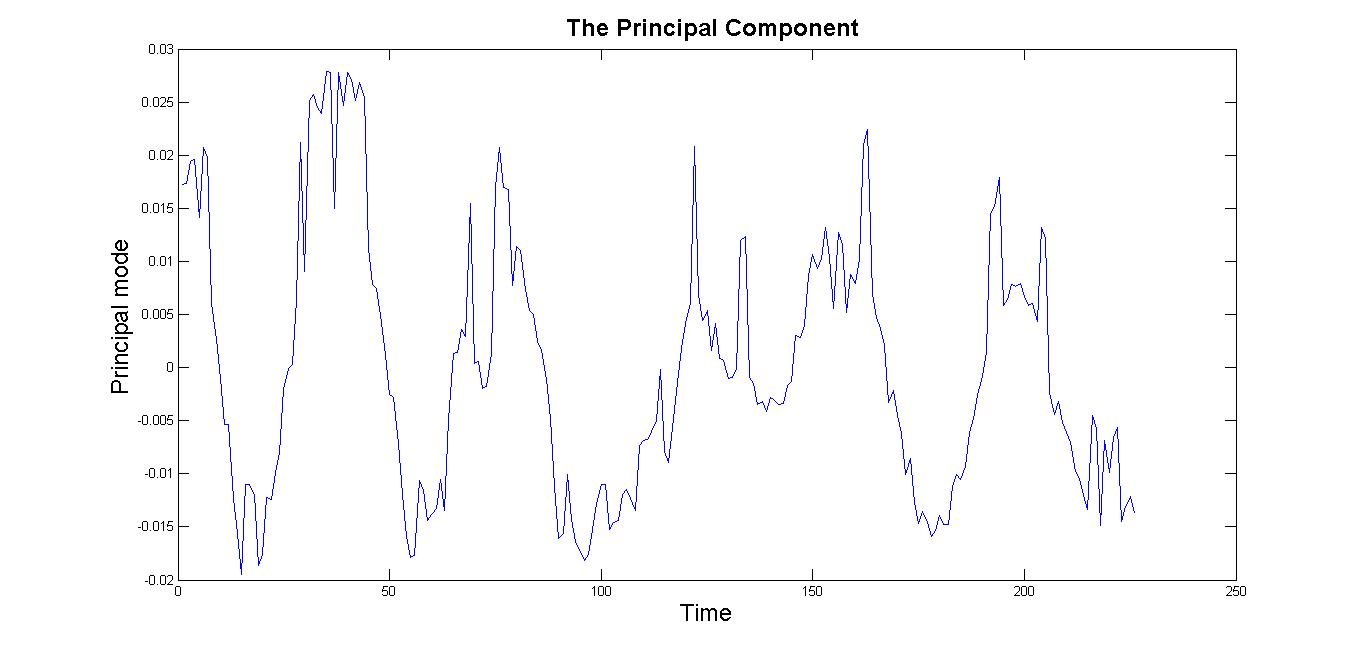
\includegraphics[width=0.6\textwidth]{PC2.jpg}
	
	\caption{The First Principal Component}	
\end{figure}
This is far from the result we obtained in the previous case. The noise has taken over the data for us to derive much insight.

\subsection{Horizontal Displacement}






\subsubsection{The Percentage of variation captured}
\begin{figure}[h!] 
	\centering
	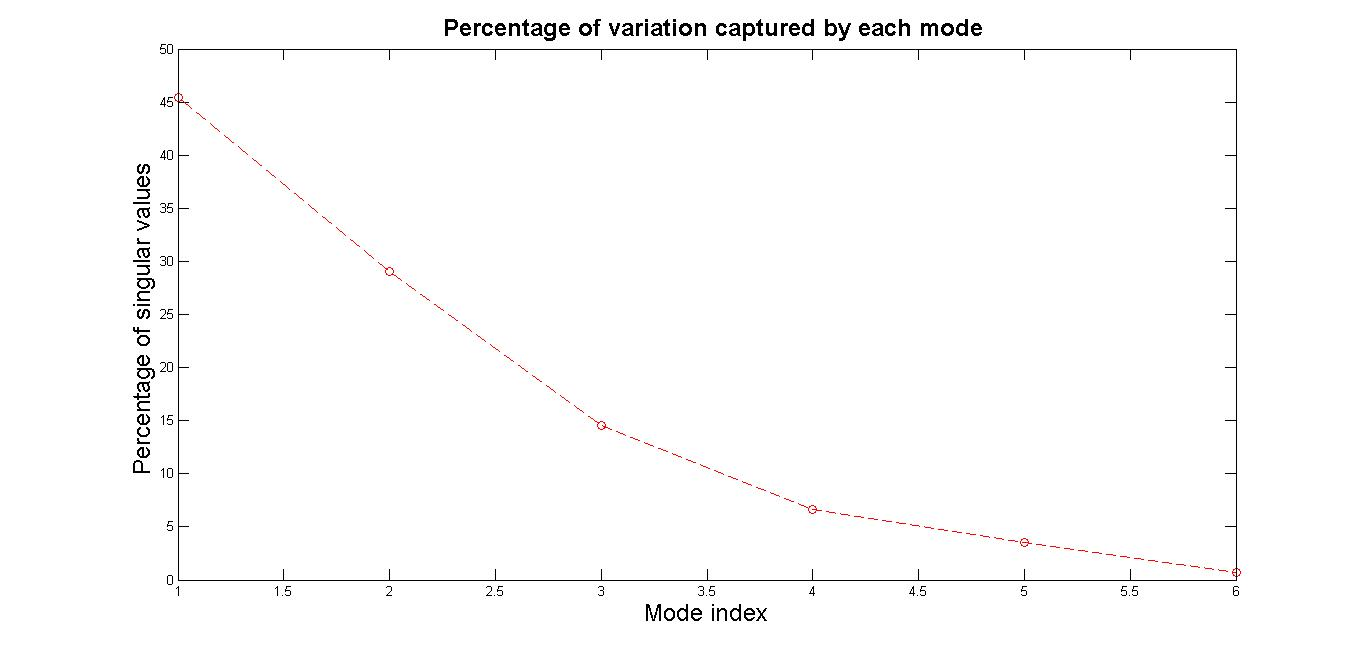
\includegraphics[width=0.7\textwidth]{percent3.jpg}
	\caption{The variation captured by each principal component}
\end{figure}

Over 45 percent of the data is captured by the first principal component. The second component has around 30 percent. So, it can't be ignored

\subsubsection{The Principal Components}
\begin{figure}[H] 
	\centering
	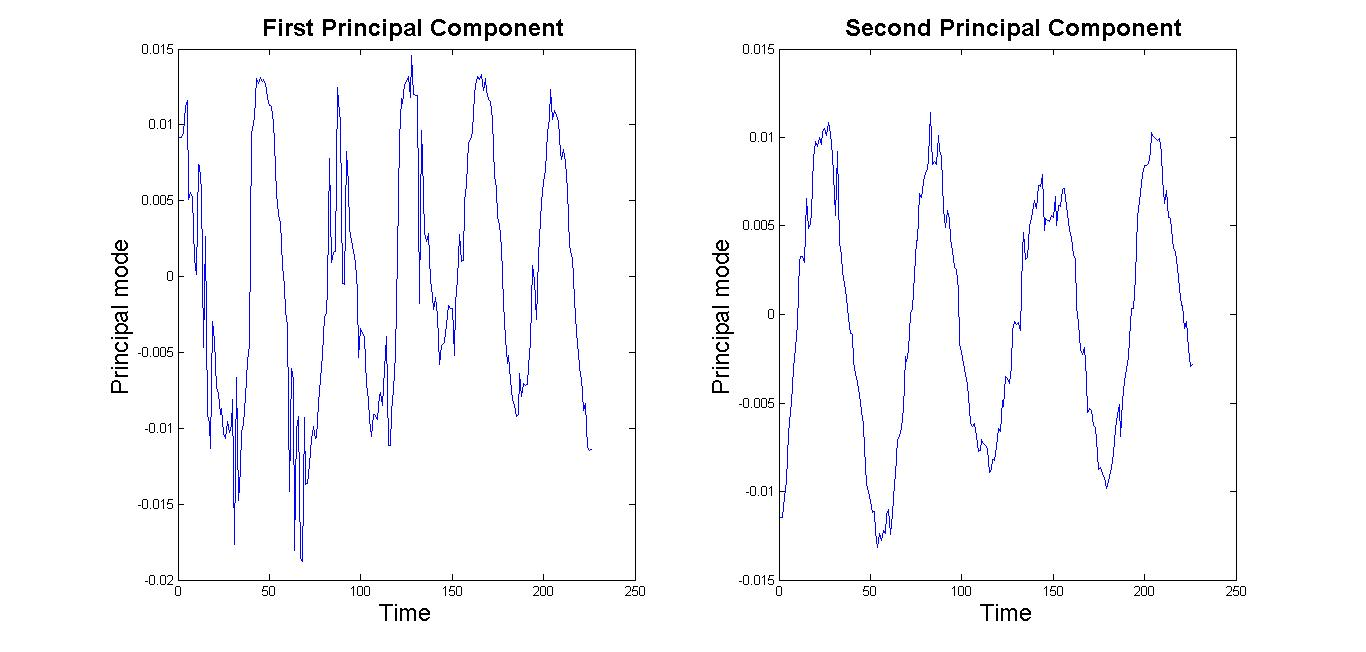
\includegraphics[width=0.8\textwidth]{PC3.jpg}
	
	\caption{The First and Second Principal Component}	
\end{figure}
Although there are a few spikes, this shows oscillations in two orthogonal directions.

\subsection{Horizontal Displacement and Rotation}







\subsubsection{The Percentage of variation captured}
\begin{figure}[h!] 
	\centering
	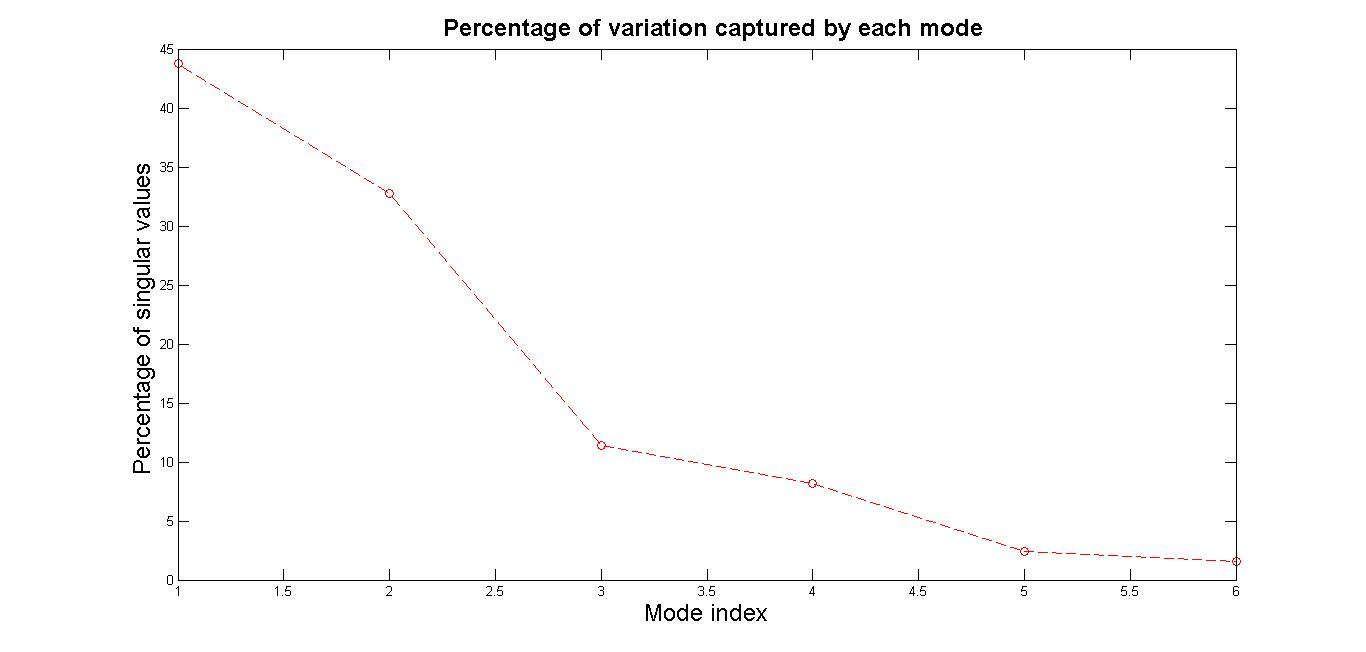
\includegraphics[width=0.7\textwidth]{percent4.jpg}
	\caption{The variation captured by each principal component}
\end{figure}

Over 45 percent of the data is captured by the first principal component and 35 percent is in the second component. 

\subsubsection{The Principal Components}
\begin{figure}[H] 
	\centering
	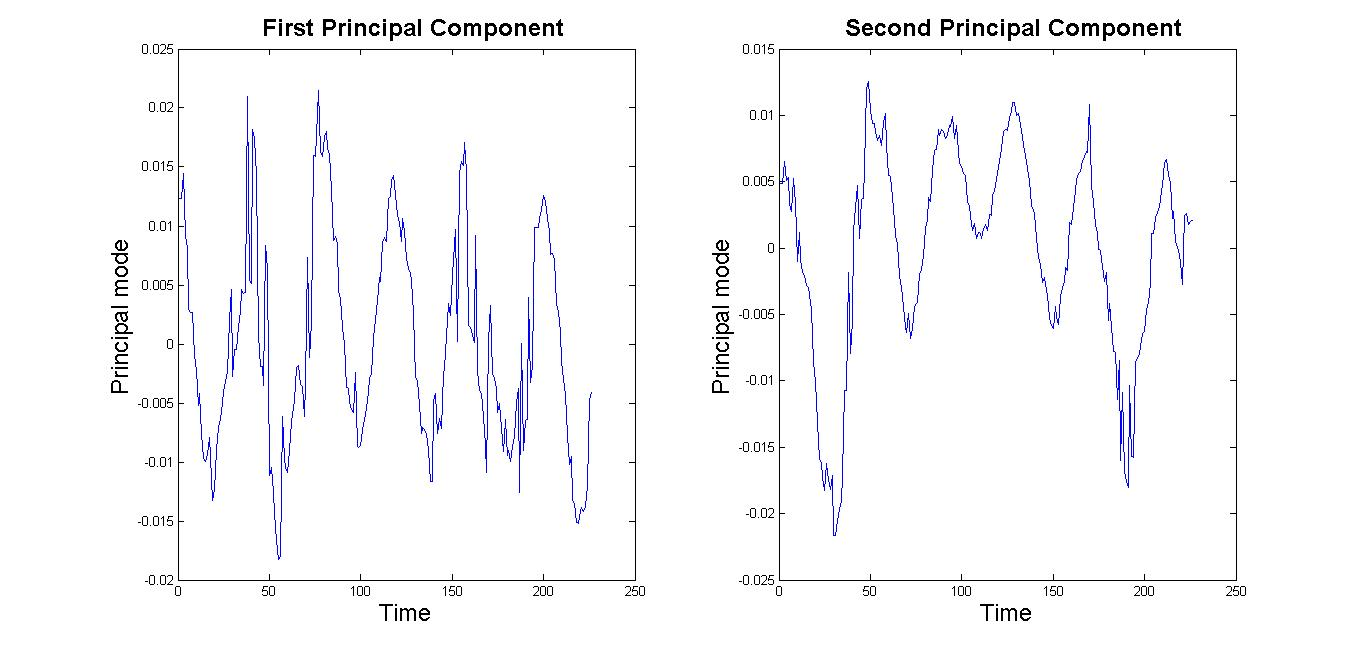
\includegraphics[width=0.7\textwidth]{PC4.jpg}
	
	\caption{The First and Second Principal Components}	
\end{figure}
These show damped oscillations in two orthogonal directions.
\section{Summary and Conclusions}
The Principal Component Analysis is a valuable tool to understand the dynamics of unknown phenomena through a mere optimal matrix transformation. We obtained the following conclusions.

\begin{itemize}
\item The PCA works well to isolate the dynamics of systems
\item However, it depends on the format of the input data. Two motions that seem orthogonal may actually a single in a different frame of reference. (like the Ferris wheel example) 
\item The PCA loses accuracy with noise.
\item Superposition of motions leads to principal components which are not small enough to ignore, like in the last two cases.	
\end{itemize}

\newpage

\appendix
%dummy comment inserted by tex2lyx to ensure that this paragraph is not empty


\section{MATLAB Functions used}
\begin{itemize}
\item \textbf{[U,S,V]=svd(A): } \\ This function performs the singular value decomposition of A and returns U,S and V.
\item \textbf{ceil: } \\ Finds a number greater than it which is closest to it.
\item \textbf{find: } \\ This is used to find indices in a matrix where a certain condition is met.
\item \textbf{frame2im: } \\ Converts a video frame to an image.
\item \textbf{regionprops: } \\ Enables you to find clusters of brightness in black and white images
\end{itemize}

\section{MATLAB Code}
\subsection{getmovout.m}
\begin{lstlisting}[style=myMatlabstyle]
function [mov]= getmovout(vidFrames)
for k=1:226
mov(k).cdata = vidFrames(:,:,:,k);mov(k).colormap = [];
end
\end{lstlisting}
\subsection{indexmat.m}
\begin{lstlisting}[style=myMatlabstyle]
function [w]= indexmat(a)
i= ceil(a/480);
j=a- 480*(i-1);
w=[i,j];
end
\end{lstlisting}
\subsection{loader.m}
\begin{lstlisting}[style=myMatlabstyle]
X4= frame2im(mov(1));
X4=rgb2gray(X4);
X4=double(X4);
disp(1);
l1=[];
l2=[];
disp(2);
for j=2:226
x1=frame2im(mov(j));
x=rgb2gray(x1);
x=double(x);
Y2=x-X4;
Y2(:,1:300)=0;
Y2(:,400:640)=0;
ma=0.8*max(max(Y2));
Y2(Y2<ma)=0;

y2bw=im2bw(Y2);
stats = regionprops(y2bw,'Centroid');
di=stats.Centroid;
l1=[l1,di(1)];
l2=[l2,di(2)];
imagesc(Y2); colorbar; drawnow;
end
\end{lstlisting}
\subsection{whiteedges.m}
\begin{lstlisting}[style=myMatlabstyle]
function [a1,a2,t]= whiteedges(mov,l,r,u,d,dimr)
if nargin < 6
dimr =   1;
end
a1= zeros(226,1);
a2= zeros(226,1);
for j=1:226
y=[];
X=frame2im(mov(j));
X=double(X);
X(:,1:l)=0;
X(:,r:640)=0;
X(1:u,:)=0;
X(d:480,:)=0;
w=0.988;
s= find(X(:,:,1)>w*max(max(X(:,:,1))) &X(:,:,2)>w*max(max(X(:,:,2)))& X(:,:,3)>w*max(max(X(:,:,3))) );
while isempty(s)
w=0.988*w;
s= find(X(:,:,1)>w*max(max(X(:,:,1))) &X(:,:,2)>w*max(max(X(:,:,2)))& X(:,:,3)>w*max(max(X(:,:,3))) );
end
t= indexmat(s);
%t=t(t(:,1)>200,:);
m=mode(t(:,dimr));
if dimr==1
diml=2;
else
diml=1;
end
y= t( t(:,dimr)==m,diml);
a1(j)=mean(y);
a2(j)=mean(m);
end
 	\end{lstlisting}
\subsection{mainregular.m}
 	\begin{lstlisting}[style=myMatlabstyle]
%% Regular Case
%% First Cam
load('cam1_1.mat');
mov1_1=getmovout(vidFrames1_1);
%playmov(mov1_1);
[a11_1,a21_1]=whiteedges(mov1_1,300,400,170,480);

%% Second Cam
load('cam2_1.mat');
mov2_1=getmovout(vidFrames2_1);
%playmov(mov2_1);
[a12_1,a22_1]=whiteedges(mov2_1,220,370,100,400);

%% Third Cam
load('cam3_1.mat');
mov3_1=getmovout(vidFrames3_1);
%playmov(mov3_1);
[a13_1,a23_1]=whiteedges(mov3_1,250,500,150,350,2);
 	\end{lstlisting}
 	\subsection{mainsecond.m}
 	\begin{lstlisting}[style=myMatlabstyle]
%% Second Case
%% First Cam
load('cam1_2.mat');
mov1_2=getmovout(vidFrames1_2);
%%%playmov(mov1_2);
[a11_2,a21_2]=whiteedges(mov1_2,300,420,220,420);

%% Second Cam
load('cam2_2.mat');
mov2_2=getmovout(vidFrames2_2);


%playmov(mov2_2);
[a12_2,a22_2]=whiteedges(mov2_2,200,400,150,400);

%% Third Cam
load('cam3_2.mat');
mov3_2=getmovout(vidFrames3_2);
%%
%playmov(mov3_2);

[a13_2,a23_2]=whiteedges(mov3_2,300,500,200,350,2);
 	\end{lstlisting}
\subsection{mainthird.m}
\begin{lstlisting}[style=myMatlabstyle]

 	%% Third Case
 	%% First Cam
 	load('cam1_3.mat');
 	mov1_3=getmovout(vidFrames1_3);
 	%playmov(mov1_3);
 	[a11_3,a21_3]=whiteedges(mov1_3,270,400,200,450);
 	
 	%% Second Cam
 	load('cam2_3.mat');
 	mov2_3=getmovout(vidFrames2_3);
 	
 	%playmov(mov2_3);
 	[a12_3,a22_3]=whiteedges(mov2_3,220,450,150,400);
 	
 	%% Third Cam
 	load('cam3_3.mat');
 	mov3_3=getmovout(vidFrames3_3);
 	
 	%playmov(mov3_3);
 	
 	[a13_3,a23_3]=whiteedges(mov3_3,300,500,150,350,2);

\end{lstlisting}
\subsection{mainfourth.m}
\begin{lstlisting}[style=myMatlabstyle]

%% Fourth Case
%% First Cam
load('cam1_4.mat');
mov1_4=getmovout(vidFrames1_4);
%playmov(mov1_4);
[a11_4,a21_4]=whiteedges(mov1_4,300,450,220,450);

%% Second Cam
load('cam2_4.mat');
mov2_4=getmovout(vidFrames2_4);
%playmov(mov2_4);
[a12_4,a22_4]=whiteedges(mov2_4,200,420,150,350);

%% Third Cam
load('cam3_4.mat');
mov3_4=getmovout(vidFrames3_4);
%playmov(mov3_4);
[a13_4,a23_4]=whiteedges(mov3_4,320,480,150,250,2);

\end{lstlisting}
\subsection{mainfourth.m}
\begin{lstlisting}[style=myMatlabstyle]
%clc; clear all; close all;
n=226;
f=18;
main_regular;
figure(1);
subplot(3,2,1);
plot(a11_1);
xlabel('Time','FontSize', f-3) % x-axis label
ylabel('Displacement','FontSize', f) % y-axis label
title(' \bf Cam 1: X direction','FontSize', f)
subplot(3,2,2);
plot(a21_1);
xlabel('Time','FontSize', f) % x-axis label
ylabel('Displacement','FontSize', f) % y-axis label
title(' \bf Cam 1: Y direction','FontSize', f)
subplot(3,2,3);
plot(a12_1);
xlabel('Time','FontSize', f) % x-axis label
ylabel('Displacement','FontSize', f) % y-axis label
title(' \bf Cam 2: X direction','FontSize', f-3)
subplot(3,2,4);
plot(a22_1);
xlabel('Time','FontSize', f) % x-axis label
ylabel('Displacement','FontSize', f) % y-axis label
title(' \bf Cam 2: Y direction','FontSize', f)
subplot(3,2,5);
plot(a13_1);
xlabel('Time','FontSize', f) % x-axis label
ylabel('Displacement','FontSize', f) % y-axis label
title(' \bf Cam 3: X direction','FontSize', f)
subplot(3,2,6);
plot(a23_1);
xlabel('Time','FontSize', f) % x-axis label
ylabel('Displacement','FontSize', f) % y-axis label
title(' \bf Cam 3: Y direction','FontSize', f)

X1=[a11_1/max(a11_1),a21_1/max(a21_1),a12_1/max(a12_1),a22_1/max(a22_1),a13_1/max(a13_1),a23_1/max(a23_1)];
mn =mean(X1,1);
X1=X1-repmat(mn,n,1);
[u1,s1,v1]=svd(X1/sqrt(n-1),'econ');
lambda1=diag(s1).^2;
percent1= lambda1*100/sum(lambda1);
figure(2);
plot(percent1, 'ro');
xlabel('Mode index','FontSize', f) % x-axis label
ylabel('Percentage of singular values','FontSize', f) % y-axis label
title(' \bf Percentage of variation captured by each mode','FontSize', f)

T1=u1*s1;
figure(3);
plot(T1(:,1), 'b');
xlabel('Time','FontSize', f) % x-axis label
ylabel('Principal mode','FontSize', f) % y-axis label
title(' \bf The Principal Component','FontSize', f)
disp(1);

main_second;
figure(4);
subplot(3,2,1);
plot(a11_2);
xlabel('Time','FontSize', f-3) % x-axis label
ylabel('Displacement','FontSize', f) % y-axis label
title(' \bf Cam 1: X direction','FontSize', f)
subplot(3,2,2);
plot(a21_2);
xlabel('Time','FontSize', f) % x-axis label
ylabel('Displacement','FontSize', f) % y-axis label
title(' \bf Cam 1: Y direction','FontSize', f)
subplot(3,2,3);
plot(a12_2);
xlabel('Time','FontSize', f) % x-axis label
ylabel('Displacement','FontSize', f) % y-axis label
title(' \bf Cam 2: X direction','FontSize', f-3)
subplot(3,2,4);
plot(a22_2);
xlabel('Time','FontSize', f) % x-axis label
ylabel('Displacement','FontSize', f) % y-axis label
title(' \bf Cam 2: Y direction','FontSize', f)
subplot(3,2,5);
plot(a13_2);
xlabel('Time','FontSize', f) % x-axis label
ylabel('Displacement','FontSize', f) % y-axis label
title(' \bf Cam 3: X direction','FontSize', f)
subplot(3,2,6);
plot(a23_2);
xlabel('Time','FontSize', f) % x-axis label
ylabel('Displacement','FontSize', f) % y-axis label
title(' \bf Cam 3: Y direction','FontSize', f)
X2=[a11_2/max(a11_2),a21_2/max(a21_2),a12_2/max(a12_2),a22_2/max(a22_2),a13_2/max(a13_2),a23_2/max(a23_2)];
mn =mean(X2,1);
X2=X2-repmat(mn,n,1);
[u2,s2,v2]=svd(X2/sqrt(n-1),'econ');
lambda2=diag(s2).^2;
percent2= lambda2*100/sum(lambda2);
figure(5);
plot(percent2, 'ro');
xlabel('Mode index','FontSize', f) % x-axis label
ylabel('Percentage of singular values','FontSize', f) % y-axis label
title(' \bf Percentage of variation captured by each mode','FontSize', f)
T2=u2*s2;
figure(6);
plot(T2(:,1), 'b');
xlabel('Time','FontSize', f) % x-axis label
ylabel('Principal mode','FontSize', f) % y-axis label
title(' \bf The Principal Component','FontSize', f)
disp(2);


main_third;
figure(7);
subplot(3,2,1);
plot(a11_3);
xlabel('Time','FontSize', f-3) % x-axis label
ylabel('Displacement','FontSize', f) % y-axis label
title(' \bf Cam 1: X direction','FontSize', f)
subplot(3,2,2);
plot(a21_3);
xlabel('Time','FontSize', f) % x-axis label
ylabel('Displacement','FontSize', f) % y-axis label
title(' \bf Cam 1: Y direction','FontSize', f)
subplot(3,2,3);
plot(a12_3);
xlabel('Time','FontSize', f) % x-axis label
ylabel('Displacement','FontSize', f) % y-axis label
title(' \bf Cam 2: X direction','FontSize', f-3)
subplot(3,2,4);
plot(a22_3);
xlabel('Time','FontSize', f) % x-axis label
ylabel('Displacement','FontSize', f) % y-axis label
title(' \bf Cam 2: Y direction','FontSize', f)
subplot(3,2,5);
plot(a13_3);
xlabel('Time','FontSize', f) % x-axis label
ylabel('Displacement','FontSize', f) % y-axis label
title(' \bf Cam 3: X direction','FontSize', f)
subplot(3,2,6);
plot(a23_3);
xlabel('Time','FontSize', f) % x-axis label
ylabel('Displacement','FontSize', f) % y-axis label
title(' \bf Cam 3: Y direction','FontSize', f)
X3=[a11_3/max(a11_3),a21_3/max(a21_3),a12_3/max(a12_3),a22_3/max(a22_3),a13_3/max(a13_3),a23_3/max(a23_3)];
mn =mean(X3,1);
X3=X3-repmat(mn,n,1);
[u3,s3,v3]=svd(X3/sqrt(n-1),'econ');
lambda3=diag(s3).^2;
percent3= lambda3*100/sum(lambda3);
figure(8);
plot(percent3, 'ro');
xlabel('Mode index','FontSize', f) % x-axis label
ylabel('Percentage of singular values','FontSize', f) % y-axis label
title(' \bf Percentage of variation captured by each mode','FontSize', f)
T3=u3*s3;
figure(9);
subplot(1,2,1);
plot(T3(:,1), 'b');
xlabel('Time','FontSize', f) % x-axis label
ylabel('Principal mode','FontSize', f) % y-axis label
title(' \bf First Principal Component','FontSize', f)
subplot(1,2,2);
plot(T3(:,2), 'b');
xlabel('Time','FontSize', f) % x-axis label
ylabel('Principal mode','FontSize', f) % y-axis label
title(' \bf Second Principal Component','FontSize', f)
disp(3);


main_fourth;
figure(10);
subplot(3,2,1);
plot(a11_4);
xlabel('Time','FontSize', f-3) % x-axis label
ylabel('Displacement','FontSize', f) % y-axis label
title(' \bf Cam 1: X direction','FontSize', f)
subplot(3,2,2);
plot(a21_4);
xlabel('Time','FontSize', f) % x-axis label
ylabel('Displacement','FontSize', f) % y-axis label
title(' \bf Cam 1: Y direction','FontSize', f)
subplot(3,2,3);
plot(a12_4);
xlabel('Time','FontSize', f) % x-axis label
ylabel('Displacement','FontSize', f) % y-axis label
title(' \bf Cam 2: X direction','FontSize', f-3)
subplot(3,2,4);
plot(a22_4);
xlabel('Time','FontSize', f) % x-axis label
ylabel('Displacement','FontSize', f) % y-axis label
title(' \bf Cam 2: Y direction','FontSize', f)
subplot(3,2,5);
plot(a13_4);
xlabel('Time','FontSize', f) % x-axis label
ylabel('Displacement','FontSize', f) % y-axis label
title(' \bf Cam 3: X direction','FontSize', f)
subplot(3,2,6);
plot(a23_4);
xlabel('Time','FontSize', f) % x-axis label
ylabel('Displacement','FontSize', f) % y-axis label
title(' \bf Cam 3: Y direction','FontSize', f)
X4=[a11_4/max(a11_4),a21_4/max(a21_4),a12_4/max(a12_4),a22_4/max(a22_4),a13_4/max(a13_4),a23_4/max(a23_4)];
mn =mean(X4,1);
X4=X4-repmat(mn,n,1);
[u4,s4,v4]=svd(X4/sqrt(n-1),'econ');
lambda4=diag(s4).^2;
percent4= lambda4*100/sum(lambda4);
figure(11);
plot(percent4, 'ro');
xlabel('Mode index','FontSize', f) % x-axis label
ylabel('Percentage of singular values','FontSize', f) % y-axis label
title(' \bf Percentage of variation captured by each mode','FontSize', f)
T4=u4*s4;
figure(12);
subplot(1,2,1);
plot(T4(:,1), 'b');
xlabel('Time','FontSize', f) % x-axis label
ylabel('Principal mode','FontSize', f) % y-axis label
title(' \bf First Principal Component','FontSize', f)
subplot(1,2,2);
plot(T4(:,2), 'b');
xlabel('Time','FontSize', f) % x-axis label
ylabel('Principal mode','FontSize', f) % y-axis label
title(' \bf Second Principal Component','FontSize', f)
disp(4);
\end{lstlisting}
\end{document}